\section{Resultater fra Affinity diagram}
\label{ParametreDatabehandlingAffinityDiagram}
%
Den her sektion skal indeholde vores analyse af vores affinity diagram, samt billeder af det. 

Muligvis en eller anden smart oversigt over hvilke parametre vi "ender" med. Jeg ved ikke om det er her skalaerne burde indgå eller om det skal vente til den part, der handler om en næste test. 

Skriv om de kriterier, de orange post its er formuleret ud fra. Skriv hvilke kriterier vi så vælger de relevante orange post its ud fra. 

\subsection{Interagerer ikke med R}
%

%
\begin{figure}[H]
\centering
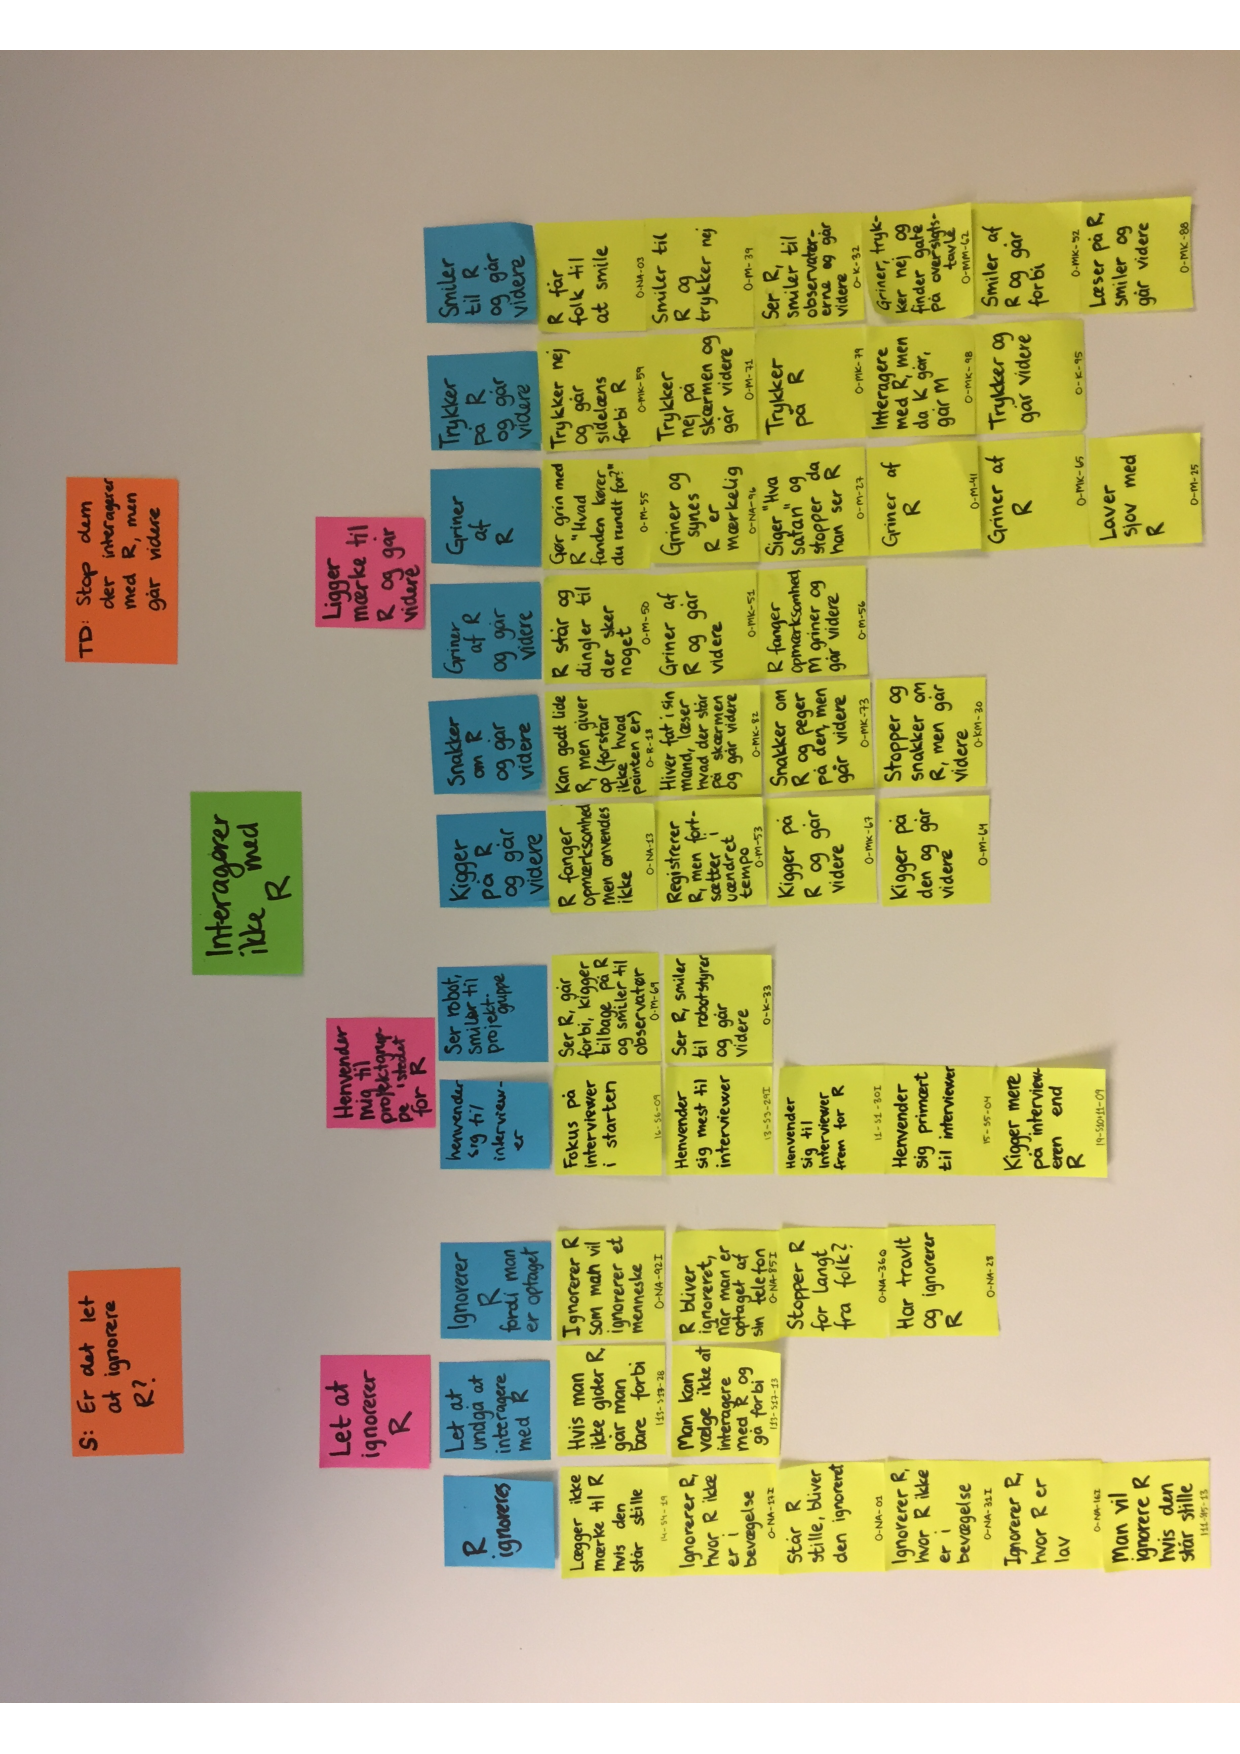
\includegraphics[width = 0.3\textwidth]{Figure/AffinityDiagram/InteragererIkkeMedR} 
\caption{Ny}
\label{fig:AFInteragererIkkeMedR}
\end{figure}
\noindent
%
Overvejelser til TD (testdesign): stop dem der interagerer med R, men som ikke har lyst til at deltage i interviewet og spørg hvorfor de ikke har lyst til at deltage. \\
S (skala): Er det let at ignorer R?/Er det let at overse R?

\subsection{Skærmen virker ikke}
%
S: Jeg synes det var svært at trykke på R's skærm\\
S: Jeg synes skærmen reagerede dårligt\\
S: Jeg synes skærmen reagerede.. (Dårligt/Godt)\\

\subsection{R kan assistere mennesker}
%
S: Jeg kan bruge R til at finde rundt i en lufthavn\\
S: Jeg føler at R kan hjælpe mig\\
S: R kan hjælpe mig så jeg ikke behøver at spørge personale\\
S: Jeg oplever R's hjælp som personlig\\
DI (Design idé): Kan hjælpe i situationer hvor jeg ikke forstår sproget. 

\subsection{R's væremåde}
%
S: Jeg oplevede R's hastighed som værende.. (Meget langsom/Meget hurtig)\\
S: Jeg synes at R's hastighed er.. (For langsom/For hurtig)\\
S: Jeg synes at R er levende\\
S: Jeg synes at R har rolige bevægelser\\
DI: Overvej om R skal tale\\
S: Jeg synes at R er irriterende\\
S: Jeg synes at R er anmassende\\
S: Jeg synes at R's bevægelser er behagelige\\
DI: R skal tilpasse sig brugerens bevægelser

\subsection{Henvendelse}
%
S: Jeg blev overrasket over R's henvendelse\\
S: Jeg synes at R stod i vejen\\
S: Jeg foretrækker at R henvender sig til mig\\
S: Jeg foretrækker at jeg henvender mig til R\\
DI: Er skal vende fronten mod den person, som R vil henvende sig til
DI: R skal være tæt på den person, som R henvender sig til\\
S: Jeg synes at R er imødekommende\\
S: Jeg synes at R kom for tæt på\\
S: Jeg synes at R er intimiderende\\

\subsection{R's udseende}
%
S: Jeg synes at R ser menneskelig ud (slet ikke menneskelig/alt for menneskelig)\\
S: Jeg foretrækker at R ser menneskelig ud\\
S: Jeg synes at R er elegant\\
S: Jeg kan godt lide R's udseende\\
DI: R skal selv indstille/tilpasse sin højde efter brugeren\\
S: Jeg oplevede R's højde som værende... (Meget lav/Meget høj)\\
S: Jeg synes at R's højde er...(For lav/For høj)\\

\subsection{Interesse for R}
%
S: R fangede min opmærksomhed\\
S: Jeg blev nysgerrig da jeg så R\\
S: Jeg synes at R er spændende\\


\subsection{Postivi overfor R}
%
S: Jeg synes R er sjov\\
S: Jeg synes R er sød\\
S: Jeg synes R er sej\\
S: Jeg synes R er nem at bruge\\
S: Jeg kan godt lide at blive betjent af R\\
S: Jeg synes R er en god idé

\subsection{Kendskab til teknologi}
%
S: Jeg har erfaring med robotter\\
S: Jeg har brug for hjælp til at bruge R\\
S: Jeg synes R minder om noget jeg kender\\
S: Min erfaring med teknologi har betydning for min oplevelse af R

\subsection{Tillid til R}
%
S: Jeg føler mig tryg ved R\\
S: Jeg regner med at R følger mig hen til det sted jeg har valgt\\
S: R gjorde mig forstrækket\\
I: Der er forskel på børn og voksnes oplevelse af R







